\documentclass[a4paper]{article}

%% Language and font encodings
\usepackage[english]{babel}
\usepackage[T1]{fontenc}

%% Sets page size and margins
\usepackage[a4paper,top=3cm,bottom=2cm,left=3cm,right=3cm,marginparwidth=1.75cm]{geometry}

%% Useful packages
\usepackage{amsmath}
\usepackage{graphicx}
\usepackage[colorlinks=true, allcolors=blue]{hyperref}

\title{Neural Networks Exercise 4}
\author{Lassi, Lehtonen 11805955\\
		Group partner: Jens, Mellberg, 11806523}

\begin{document}
\maketitle

   \begin{figure}[h]
\caption{Tanh, Learning rate: 0.2}
\centering
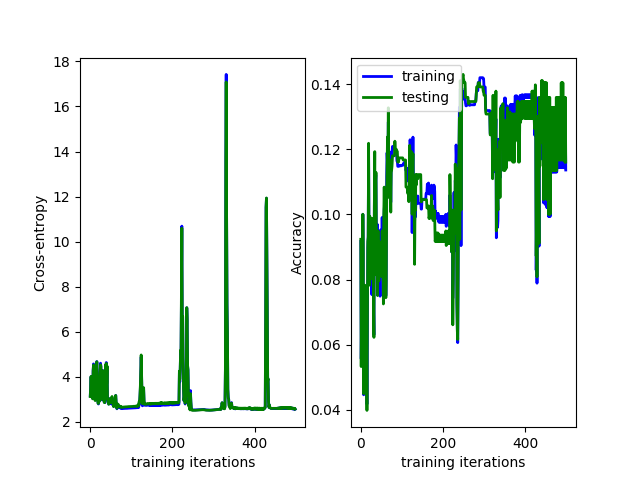
\includegraphics[width=12cm, height=10cm]{LR02.png}
\end{figure}

For this assignment we will be using a normalized data set to avoid that the training examples vary too much from eachother.\\\\
Using the tanh activation function didn't really create any surprises, an accuracy of about 0.55 seems to be the best we can achieve. Higher learning rates obviously just created more fluctuation in the graph due to the training process taking bigger steps in the error function. The final test error is significantly lower compared to using the smaller network in task 2, it also required a much smaller learning rate to achieve a good result. This strengthens the idea that a bigger network can be much harder to train efficiently. \\\\
Also as we see in the graphs, using the ReLu activation function with a too high learning rate will cause the network to get stuck with an accuracy of 0.038. We think this happens because too many neurons gets stuck with a constant output of 0 and never being able to recover, rendering the node useless. (Note that an accuracy of 0.038 is what you get by choosing a letter completely on random). But when using a very small learning rate, the accuracy slowly increases. It does take a huge amount of iterations to actually get the network to a good accuracy though and even after 1250 iterations it's only at about 0.4.\\\\
Here we see that the ResNet performs way better than the previous networks, although still only slightly better than the smaller network in Task 2. This tells us that it must be making use of the fact that it can "skip" nodes and use the previous input instead of trying to calculate a new one. 




   \begin{figure}[h]
\caption{Tanh, Learning rate: 0.5}
\centering
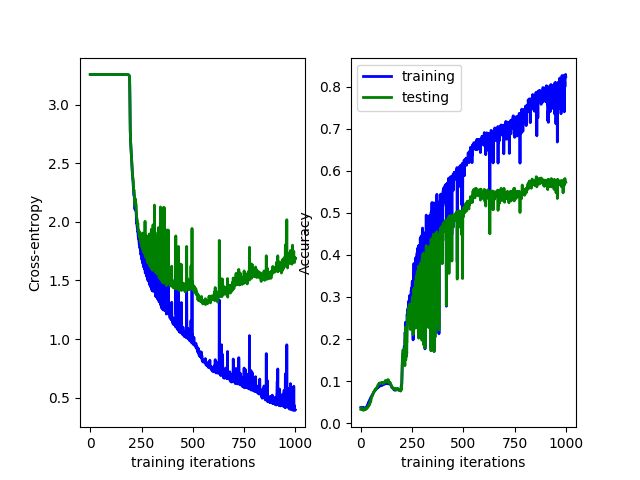
\includegraphics[width=12cm, height=10cm]{LR05.png}
\end{figure}

   \begin{figure}[h]
\caption{Tanh, Learning rate: 0.001}
\centering
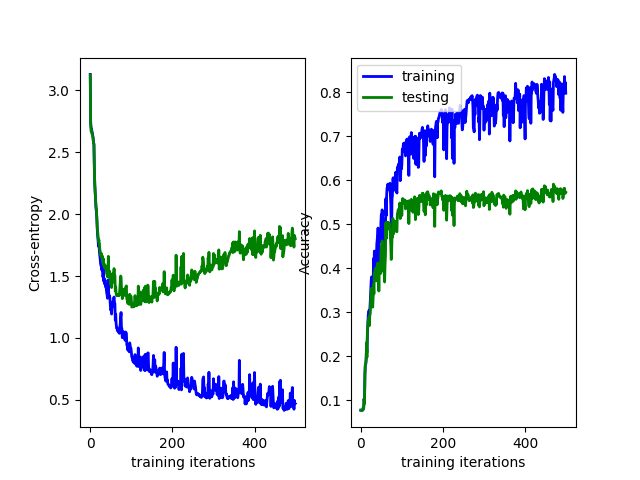
\includegraphics[width=12cm, height=10cm]{LR001.png}
\end{figure}

    

   \begin{figure}[h]
\caption{Relu, Learning rate: 0.001}
\centering
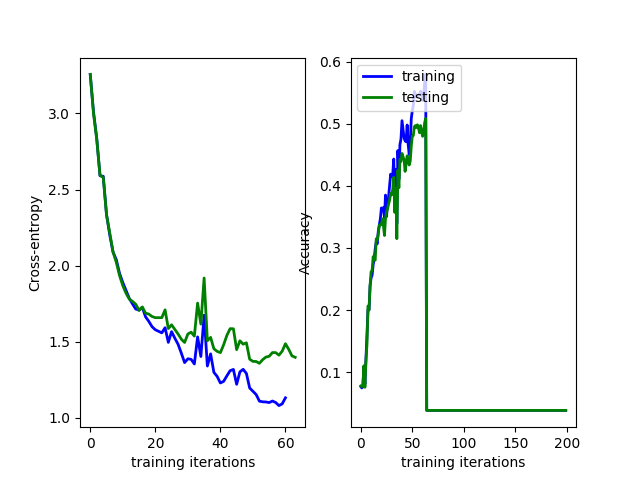
\includegraphics[width=12cm, height=10cm]{RELU001.png}
\end{figure}
    

\begin{figure}[h]
\caption{Relu, Learning rate: 0.00001}
\centering
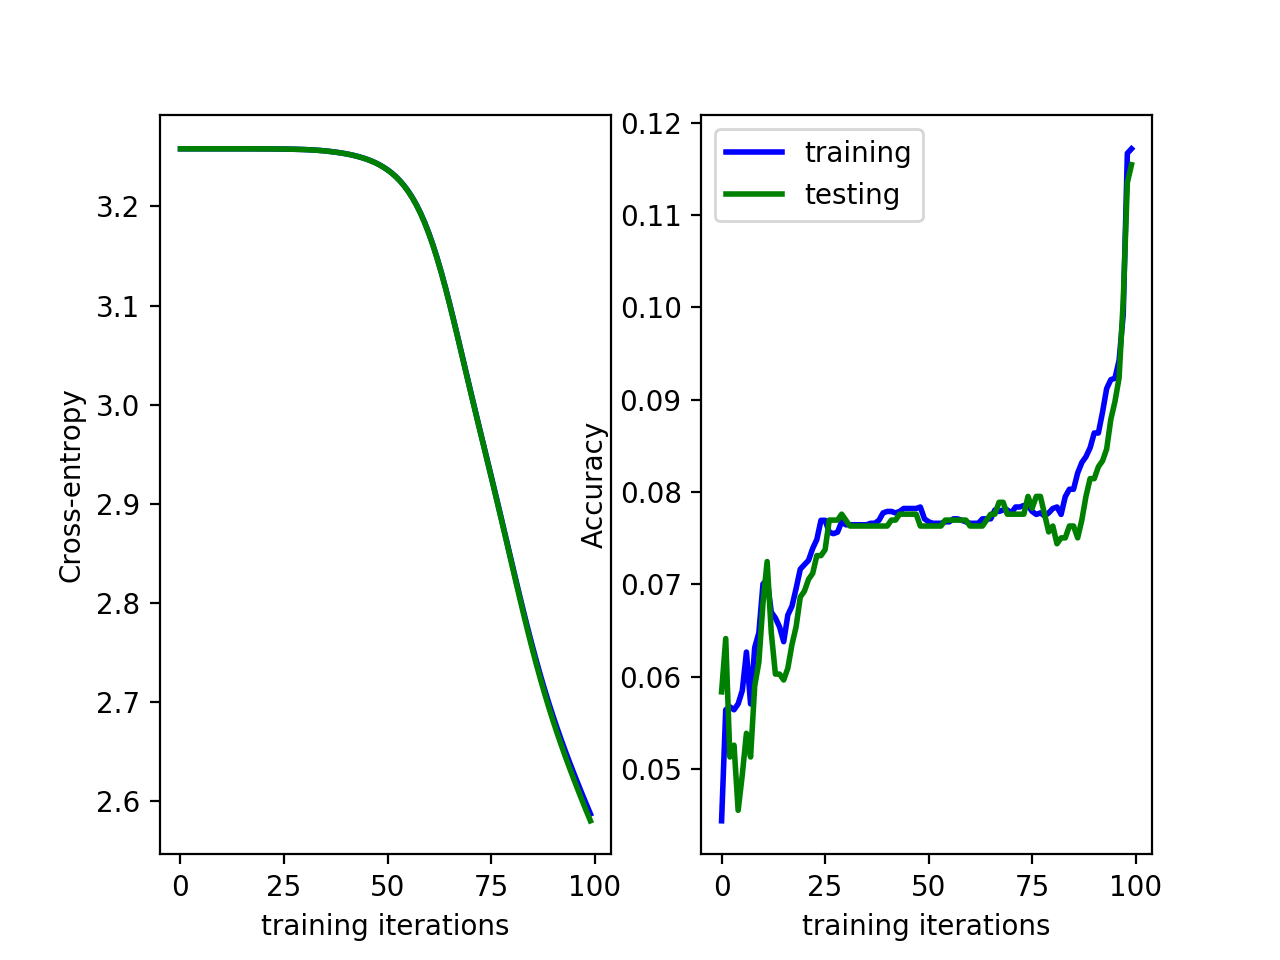
\includegraphics[width=12cm, height=10cm]{LR00001.png}
\end{figure}

\begin{figure}[h]
\caption{Relu, Learning rate: 0.00001}
\centering
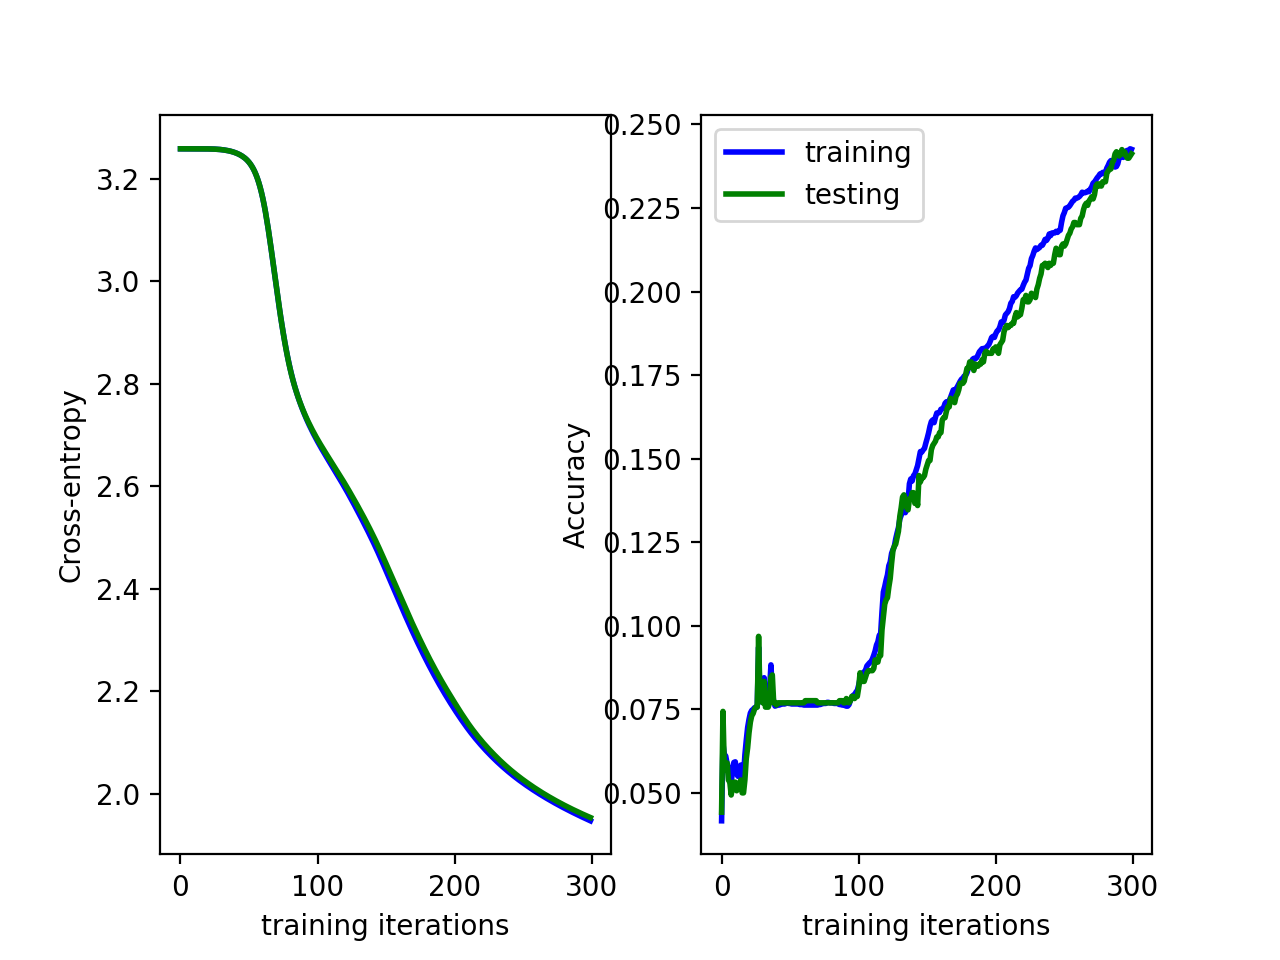
\includegraphics[width=12cm, height=10cm]{LR00001_2.png}
\end{figure}

\begin{figure}[h]
\caption{Relu, Learning rate: 0.00001}
\centering
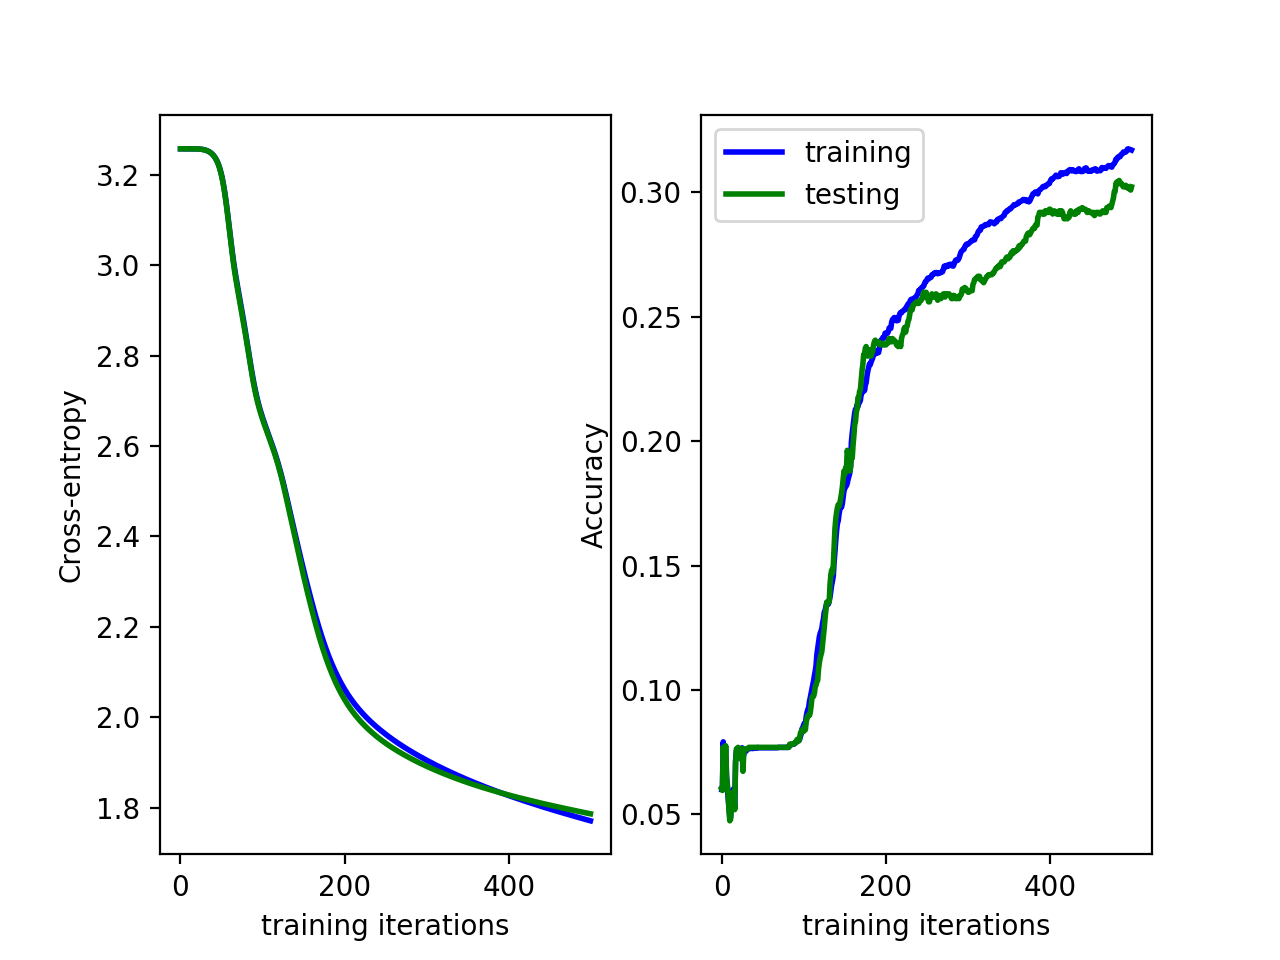
\includegraphics[width=12cm, height=10cm]{LR00001_3.png}
\end{figure}

\begin{figure}[h]
\caption{Relu, Learning rate: 0.00001}
\centering
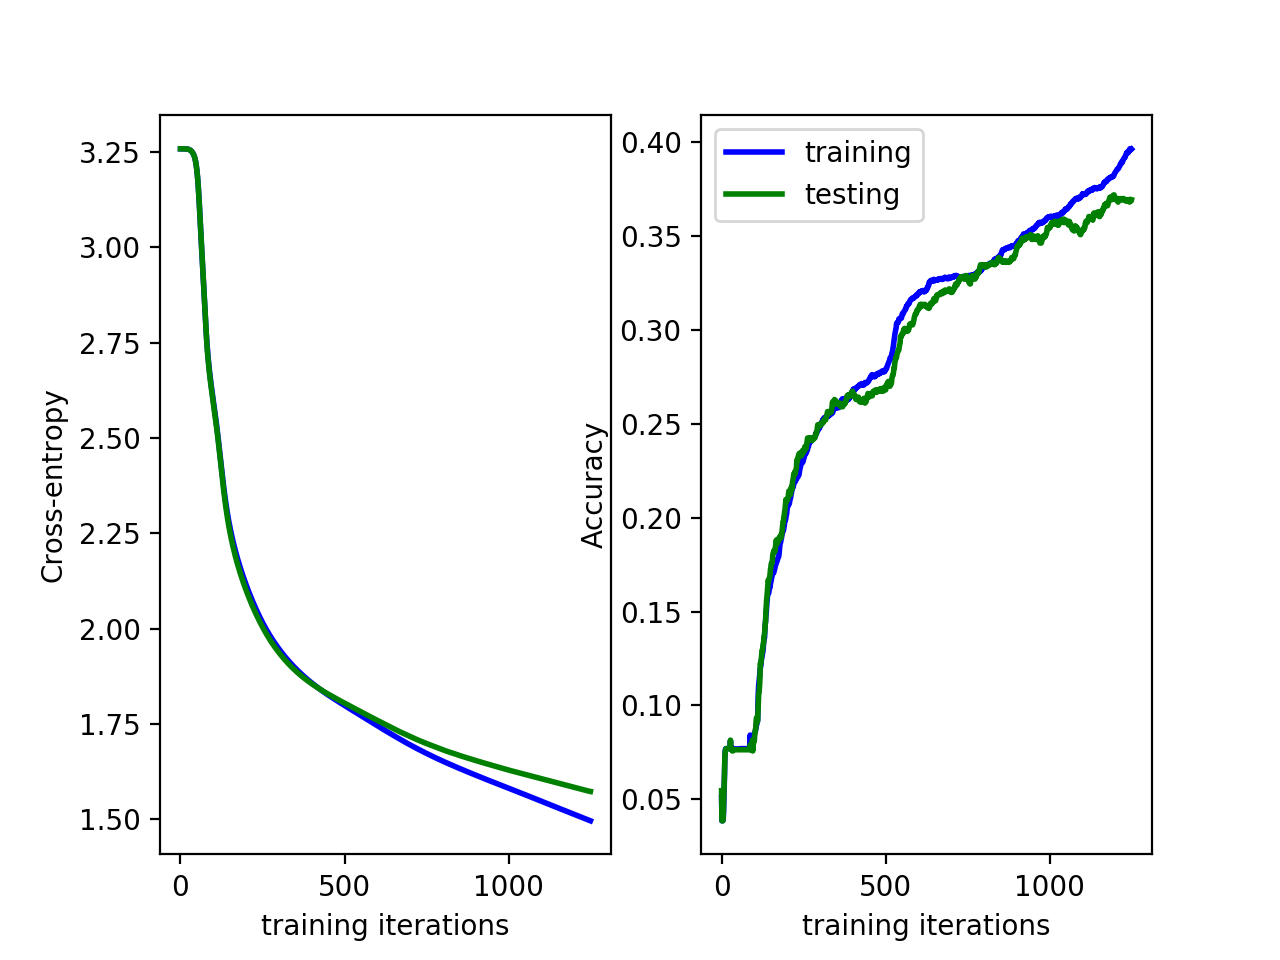
\includegraphics[width=12cm, height=10cm]{LR00001IT1250.png}
\end{figure}

\begin{figure}[h]
\caption{ResNet, Learning rate: 0.001}
\centering
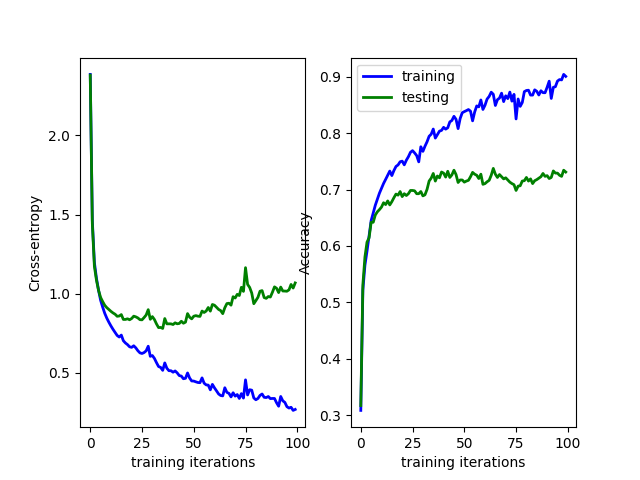
\includegraphics[width=12cm, height=10cm]{RES001.png}
\end{figure}

\begin{figure}[h]
\caption{ResNet, Learning rate: 0.00001}
\centering
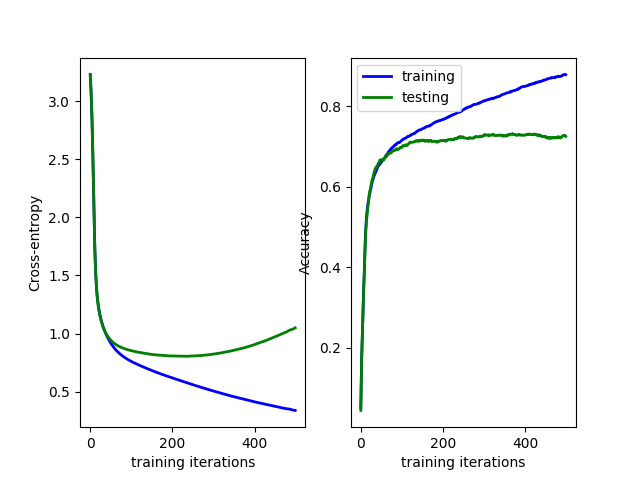
\includegraphics[width=12cm, height=10cm]{RES00001.png}
\end{figure}





\end{document}